\documentclass[a4paper,12 pt]{article}

\usepackage[T1]{fontenc}
\usepackage[polish]{babel}
\usepackage[margin=1in]{geometry}
\linespread{1.3}
\usepackage[utf8]{inputenc}
\usepackage{lmodern}
\usepackage{amsmath}
\usepackage{graphicx}
\usepackage{makeidx}
\usepackage{caption}
\usepackage{placeins}
\usepackage{listings}

\DeclareCaptionType{mycapequ}[][List of equations]
\captionsetup[mycapequ]{labelformat=empty}


\makeatletter
\setlength{\@fptop}{0pt}
\makeatother

\makeindex
\selectlanguage{polish}

\author{Rafał Cieślak}
\title{Strona tytułowa }
\date{ }

\begin{document}

\maketitle


\newpage
\tableofcontents
\listoffigures
\listoftables

\listofmycapequs

\newpage
\section{Wstęp}

\newpage
\section{Cel pracy}

\newpage
\section{Wprowadzenie teoretyczne}
\subsection{Sygnał mowy}
Mową okreslamy komunikowanie się między sobą ludzi, za pomocą ukształtowanego zbioru dźwięków i reguł, zwanego językiem.
Produkcja mowy jest wielokrokowym procesem zamiany myśli w ustną wypowiedź, która może być zarejestrowana jako sygnał mowy.
\subsubsection{Powstawanie mowy}

Sygnal mowy ludzkiej jest sygnałem akustycznym powstającym podczas przepływu powietrza poprzez aparat mowy, który jest definiowany jako 3 osobne grupy narządów. 
Składowymi aparatu mowy są:
\begin{enumerate}
\item Aparat oddechowy. Bierze udział w początkowej fazie powstawania mowy, dostarczając kolejnym składowym strumień powietrza, który jest niezbędny do wygenerowania drgań. Dzieje się to podczas wydechu. Elementy, z których jest zbudowany to płuca, oskrzela, przepona oraz tchawica.

\item Aparat fonacyjny, którego głównym elementem jest krtań. Jest to narząd niezbędny do wygenerowania jakiegokolwiek dźwięku, nie tylko mowy. Najważniejszym elementem krtani, w kontekście procesu powtarzania dźwięku, są fałdy głosowe. W ich skład wchodzą więzadła głosowe oraz mięśnie głosowe. Przestrzeń pomiędzy nimi nazywana jest szparą głośni. Struktury te przybliżają się i oddalają od siebie podczas powstawania dźwięku co powoduje zwarcie i rozwarcie szpary głośni. Podczas oddychania oraz przy generowaniu głosek bezdźwięcznych, fałdy są rozsunięte, natomiast zwierają się  i rozwierają podczas powstawania głosek dźwięcznych. 

\begin{figure}[!htbp]

\centering
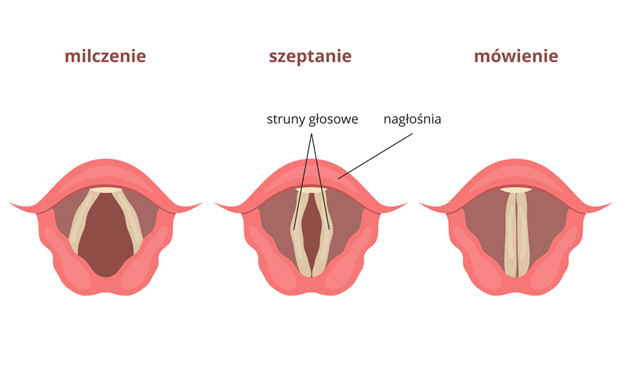
\includegraphics{faldy_glosowe}
\caption{Fałdy głosowe}

\end{figure}
\FloatBarrier

Dzięki tej czynności, strumień powietrza wprowadzany jest w drgania, co postrzegamy jako dźwięczność. Cecha ta występuje wraz z każdą samogłoską oraz przy niektórych spółgłoskach. Podczas drgań generowany jest ton krtaniowy, zwany również częstotliwością podstawową, oznaczany w literaturze jako F0. 
\item Aparat artykulacyjny, w którego skład wchodzą jamy przewodu oddechowego, znajdującego się ponad krtanią. Najważniejsze z punktu widzenia artykulacji - nosowa, gardłowa oraz ustna - nazywane są nasadą. Artykulatory znajdujące się w nasadzie dzielone są na ruchome oraz nieruchome. Do ruchomych zaliczamy język, podniebienie miękkie, wargi oraz żuchwę. Nieruchomymi określamy zęby, dziąsła oraz podniebienie twarde. Ich ustawienie ostatecznie determinuje cechy wytwarzanego dźwięku. 
\end{enumerate}

\subsubsection{Rejestrowanie sygnału mowy}

Dźwięk opuszczający aparat mowy może zostać zarejestrowany przez mikrofon w celu poddania szczegółowej analizie. Aby możliwe było przetwarzanie sygnału przez program komputerowy, konieczne jest przetworzenie sygnału z postaci analogowej do cyfrowej. W tym celu pobiera się próbki sygnału. Wartość określającą ilość próbek w jednostce czasu nazywamy częstotliwością próbkowania. Najczęściej spotykana wartość to 44,1 kHz. Oznacza to, że podczas sekundy pobierane jest 44100 wartości sygnału ciągłego. Liczba ta została przyjęta jako standard przy nagrywaniu audio na płytach CD. Tak pobrane próbki, po poddaniu procesowi kwantyzacji, tworzą sygnał cyfrowy.
Sygnał dźwiękowy może być nagrywany w wersji monofonicznej lub stereofonicznej. Oznacza to użycie jednego lub dwóch (lewy,prawy) kanałów. Nagrania rejestrowane tymi sposobami różnią się od siebie diametralnie, zarówno w kontekście subiektywnych odczuć słuchacza, jak i podczas przetwarzania sygnału. Kanały w wersji stereofonicznej mogą róźnić się od siebie wartościami próbek, zwłaszcza w widmie sygnału.

\subsubsection{Parametryzacja}

Po uzyskaniu sygnału cyfrowego, w dalszym toku analizy dźwięku, podejmowane są kroki przygotowawcze do parametryzacji, zwane przetwarzaniem wstępnym. 




Między innymi usuwana jest cisza z początku i końca nagrania oraz przeprowadzana jest normalizacja. 

Normalizacja może być przeprowadzona na dwa sposoby. Jeden z nich polega na  uzyskaniu próbki o największej wartości w całym sygnale, a następnie podzieleniu wszystkich próbek przez tą maksymalną wartość. Zbiór nowych wartości będzie się mieścił w przedziale <-1;1>.
 Innym podejsciem jest podzielenie próbek sygnału przez maksymalną wartosc ich typu. 
\begin{figure}[h]

\centering
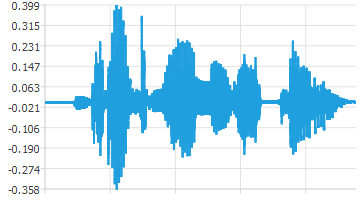
\includegraphics{stol_waveform}
\caption{Nagranie słów "drewniany stół". Sygnał po normalizacji, przed usunięciem ciszy}

\end{figure}
\FloatBarrier
Najczęsciej oznacza to podzielenie przez 32167, jako że jest to maksymalna wartosć typu short int, zazwyczaj używanego do przechowywania próbek sygnału.
Jako jeden z kroków przetwarzania wstępnego stosowana jest również filtracja preemfazy, której celem jest uwypuklenie wysokich częstotliwości kosztem składowych o niskich częstotliwościach.
\begin{mycapequ}[h]

\begin{equation}
x_{n}'=x_{n} - a*x_{n-1}       
\end{equation}
\caption{Filtracja preemfazy,  a=0.97 }
\end{mycapequ} 
\FloatBarrier
Ostatnim etapem przetwarzania wstępnego jest segmentacja, zwana również ramkowaniem. Sygnał jest dzielony na 20 milisekundowe ramki (frames). Ramki nachodzą na siebie, w celu uniknięcia utraty jakichkolwiek danych (overlapping). Wielkość zachodzenia powinna wynosić co najmniej 1/3 dlugości ramki. Tak przygotowany sygnał może być poddany parametryzacji, zwanej inaczej ekstrakcją cech. 
Proces ten ma na celu uzyskanie wektora parametrów dotyczących ramki sygnału.
\newline Parametry dzielimy na czasowe i widmowe.
Do cech czasowych zalicza się:
\begin{enumerate}
\item Energia, będaca sumą wszystkich próbek w danej ramce, podniesionych do kwadratu. Jest istotną cechą w procesie mającym na celu rozpoznanie mówcy.
\newline Obliczana wzorem:
\begin{mycapequ}[h]
\begin{equation}
\sum\limits_{i=0}^{W} x_{i}^2
\end{equation}
\caption{Energia sygnału, W= liczba próbek w ramce}
\end{mycapequ} 
\FloatBarrier

\begin{figure}[h]

\centering
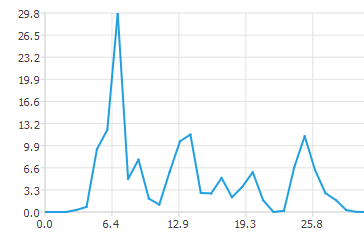
\includegraphics{energia.png}
\caption{Rozkłąd energii dla przykładowego nagrania słów "drewniany stół"}

\end{figure}
\FloatBarrier

\item Zero-crossing rate - ilosć przejsć przez zero (pare zdan do dodania w tym miejscu)

\end{enumerate}

Znacznie więcej korzyści można zyskać analizując widmowe parametry. Najpierw jednak konieczne jest uzyskanie widma sygnału, które najczęściej obliczane jest przy użyciu szybkiej transformaty Fouriera (FFT). Sygnał w takiej postaci może zostać poddany analizie częstotliwościowej.
\begin{figure}[h]

\centering
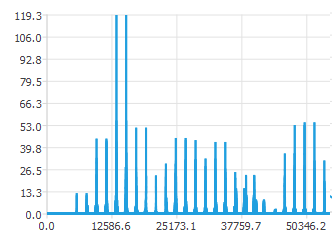
\includegraphics{fft.png}
\caption{Przebieg widma sygnału dla przykładowego nagrania słów "drewniany stół"}

\end{figure}
\FloatBarrier



\subsection{Ton podstawowy}

\subsubsection{Definicja tonu podstawowego}
W literaturze własnosć bywa również nazywana częstotliwoscią podstawową lub po prostu oznaczana jest jako F0.W zależności od potrzeb, ton podstawowy bywa różnie definiowany. W kontekście przetwarzania sygnału  mowy rozumiany jest jako wibracje strun głosowych, towarzyszące powstawaniu głosek dźwięcznych. Przebieg częstotliwości podstawowej w dużym stopniu odzwierciedla intonację wypowiedzi. Pełni istotną funkcję w językach tonalnych, w których wielu słów jest zapisywanych tak samo, a jedynie nadawany im ton pozwala rozróżnić ich znaczenie. Z tego powodu też poprawna estymacja F0 jest konieczna w systemach rozpoznawania mowy dla języków tonalnych.
Dla idealnie okresowego sygnału, częstotliwość podstawowa byłaby po prostu odwrotnością okresu. Jednak sygnał mowy jest sygnałem bardzo dynamicznym, co sprawia, że estymacja F0 przestaje być zadaniem trywialnym. Dodatkowo transformacja sygnału analogowego do postaci dyskretnej, wiążąca się zawsze z utratą danych oraz towarzyszący nagranemu głosowi szum wpływają negatywnie na dokładność estymacji. 
\subsubsection{Przegląd metod estymacji}
Prowadzone badania nad częstotliwością podstawową doprowadziły do wynalezienie wielu algorytmów estymacji o różnej skuteczności, zarówno w dziedzinie czasowej jak i widmowej.
Przykłady metod czasowych:
\begin{enumerate}
\item Analiza funkcji autokorelacji, polegająca na badaniu korelacji między danymi wejściowymi sygnału przy różnych opóźnieniach. Implikuje to wiele operacji mnożenia oraz dodawania. Estymacja F0 z wykorzystaniem tej metody związana jest z wykrywaniem maksimów lokalnych funkcji autokorelacji.
\item AMDF (Average Magnitude Difference Function) będąca odmianą funkcji autokorelacji. Polega na analizie relacji sygnału do jego opóźnionej w czasie wersji. Jako, że nie występują tu operacje mnożenia, złożoność czasowa tego algorytmu jest niższa.
\end{enumerate}
Przykładem metody widmowej jest metoda cepstralna.
,,W metodzie tej obliczana  jest odwrotna transformata Fouriera logarytmu widma amplitudowego analizowanej ramki sygnału wg wzoru:''
Dzięki analizie pozycji maksimum w dziedzinie cepstralnej, możliwe jest oszacowanie F0.




\subsubsection{Definicja algorytmu YIN}

Metody widmowe umożliwiały lepszą dokładność estymacji częstotliwości podstawowej, do momentu opracowania algorytmu YIN. W podstawowej wersji bazuje na analizie funkcji autokorelacji w dziedzinie czasu. Jego autorami są Hideki Kawahara oraz Alain de Cheveigne, którzy zaprezentowali te podejście w 2002 roku. Algorytm ten posiada kilka własności, dających mu przewagę nad konkurencyjnymi metodami. Nie posiada górnego limitu frekwencji, dla których działa poprawnie, dzięki czemu wyniki nie są zakłamywane dla wysokich głosów. Ta cecha jest również znacząca w użyciu algorytmu do analizy muzyki. Ważną własnością jest fakt, że algorytm ten jest relatywnie prosty, co pozwala na efektywną implementację, bez dużych opóźnień. Na jego prostotę istotnie wpływa niewielka liczba wymaganych parametrów.

\subsubsection{Porównanie algorytmu z konkurencyjnymi metodami}
Najważniejszą własnoscią algorytmu jest bardzo niska stopa błędów.
\begin{figure}[h]

\centering
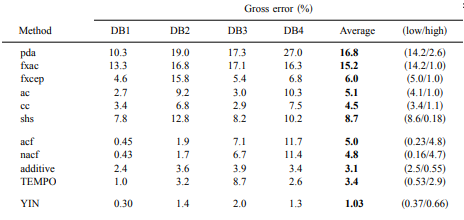
\includegraphics{porownanie_metod.png}
\caption{Wyniki porównania metod estymacji, dokonanego przez twórców algorytmu YIN}

\end{figure}
\FloatBarrier

 Do oszacowania stopy błędów autorzy algorytmu użyli laryngografu – urządzenia, które umożliwia rejestrowanie wibracji strun głosowych, za pomocą elektrod umieszczanych na krtani. Jako błędne uznawane były wartości uzyskane za pomocą każdej z metod, które różniły się o więcej niż 20 procent od wartości uzyskanych za pomocą laryngografu. Wyniki porównano dla 11 różnych metod, działających zarówno w dziedzinie czasowej, jak i widmowej. Testowane były dla różnych baz nagrań. 

Pierwsza baza (DB1) zawiera 14 głosów męskich oraz 14 głosów żeńskich, każda z osób wypowiedziała 30 zdań w języku japońskim. Na drugą bazę składa się 1 głos męski oraz 1 głos żeński, obie osoby wypowiedziały 50 zdań w języku angielskim. Trzecią bazę stanowią nagrania 2 kobiet oraz 2 mężczyzn, wypowiadających po 50 zdań w języku francuskim. Czwarta baza składa się ze zdań oraz pojedynczych słów, nagranych przez 2 mężczyzn posługujących się językiem angielski oraz mężczyznę i kobietę, używających języka japońskiego.Wyniki mniejsze od 20 \% od wartości prawidłowych sklasyfikowane zostały jako low errors, oraz jako high errors w przeciwnym przypadku. Średnia stopa błędów algorytmu YIN okazała się niższa 3-krotnie od najlepszych z pozostałych metod oraz 5-krotnie od funkcji autokorelacji, na której algorytm ten jest bazowany. Funkcja autokorelacji zbyt często zawyżała wynik (high = 4.8). 
Stopień błędów zależy od ustalonego progu tolerancji. Dla progu 20 \% stopa błędów dla YIN wynosi 1\%, dla progu 5\% wynik ten wynosi 6\%, a gdy poprzeczka zostaje obniżona do 1\%, YIN wciąż myli się tylko w 40\% przypadków, co jest również wynikiem zdecydowanie lepszym od pozostałych metod.
Wyniki otrzymane dla wąskiego zakresu częstotliwości mogłyby się różnić nieznacznie na korzyść innych metod, mogących się w takowych specjalizować, jako że badanie te zostało wykonane dla szerokiego zakresu częstotliwości (40 – 800 Hz).



\subsubsection{Opis działania algorytmu}
\begin{enumerate}
\item Pierwszym krokiem algorytmu jest obliczenie funkcji różnicowej, będącej zmodyfikowaną wersją funkcji autokorelacji. Maksima lokalne (w literaturze anglojęzycznej określane jako „peaks”) znajdywane są za pomocą wzoru:

\begin{mycapequ}[h]

\begin{equation}
d_{t}(\tau)=r_{t}(0)+r_{t+\tau}(0) - 2*r_{t}(\tau)       
\end{equation}
\caption{Funkcja różnicowa}
\end{mycapequ} 
\FloatBarrier
We wzorze tym  rt (0) jest sumą podniesionych do kwadratu wartości sygnału, obliczaną w następujący sposób:

\begin{mycapequ}[h]
\begin{equation}
\sum\limits_{i=0}^{W-1} x_{i}^2
\end{equation}
\caption{Pierwszy element równania funkcji różnicowej}
\end{mycapequ} 
\FloatBarrier

Literą W w tych wzorach oznaczona jest połowa ilosci próbek w ramce. Kolejny element zawarty w głównym wzorze, r$_{\text{t+$\tau$}}$(0) obliczany jest na bazie r$_{\text{t}}$ wg wzoru:

\begin{mycapequ}[h]
\begin{equation}
\sum\limits_{i=1}^{W-1} r_{i-1}-x_{i-1}^2+x_{i+W}^2
\end{equation}
\caption{Drugi element równania funkcji różnicowe}
\end{mycapequ} 
\FloatBarrier
Ostatnią składową potrzebną do obliczenia wartości funkcji różnicowej jest podwojone  r$_{\text{t}}$
Dla lepszych rezultatów wartość ta może zostać obliczone z wykorzystaniem szybkiej transformaty Fouriera.
Krok ten jest ma największy wpływ na obniżanie stopy błędów estymacji. Wyniki uzyskane po pierwszym etapie algorytmu już są znacząco dokładniejsze w porównaniu do wartości uzyskanych za pomocą czystej funkcji autokorelacji. Wpływ ma na to fakt, że autokorelacja ma tendencję do zawyżania wartości maksimów lokalnych wraz ze wzrostem wartości czasu. W funkcji różnicowej tendencja ta również występuje, choć w znacznie mniejszym stopniu i dotyczy sytuacji odwrotnej, zaniżania wartości maksimów.

\item Aby zlikwidować te zaburzenia wyniki uzyskane za pomocą funkcji różnicowej poddawane są modyfikacji. Stosowana jest normalizacja skumulowana, której celem jest uśrednienie bieżącej wartości przez sumę poprzedzających wartości, podzielonych przez wartość bieżącego opóźnienia. Krok ten sprawia, że YIN nie posiada górnego limitu częstotliwości.
\begin{gather*}
d_{t}'(\tau) =
\begin{cases}
  1,  \text{if }\tau=0 \\
  d_{t}(\tau)/[ (1/\tau) * \sum\limits_{j=1}^{\tau}d_{t}(j)]
\end{cases}
\end{gather*}
\item Wartość progowa. Ten krok wraz z poprzednim odpowiedzialne są za ukierunkowanie algorytmu na poszukiwanie minimum, co jest przeciwieństwem do założeń funkcji autokorelacji. Algorytm wyszukuje pierwsze minimum lokalne, którego wartość jest mniejsza od ustalonego progu. Próg ten najczęściej wynosi 0.1 lub 0.15. Jeśli takie minimum nie istnieje, zamiast niego zwracane jest minimum globalne. Jest to kolejny krok w redukowaniu stopy błędów. Zmniejsza znacząco występowanie błędów zbyt niskiej estymacji.

\item Interpolacja paraboliczna. Stosuje się interpolowanie wartości pomiędzy próbkami otaczającymi znalezione minimum, aby znaleźć prawdziwe opóźnienie, nie będące liczbą całkowitą, dla którego minimum wystąpiło. Krok ten ma niewielki wpływ na ogólny rezultat działań, jednak wpływ ten wciąż może być istotny w niektórych zastosowaniach.
\item Estymacja lokalna
\end{enumerate}
Na podstawie tak wyestymowanego tonu podstawowego, można dokonać analizy intonacji.
\subsection{Intonacja}
Intonacja jest zmianą tonu podstawowego, nie wpływającą na rozpoznawanie słów. Jest jedną z trzech głównych brzmieniowych właściwości mowy, obok akcentu i iloczasu. Najczęściej jest dodawana podczas wypowiedzi w celu oddania emocji. W wielu językach, w tym także w polskim, nadawanie wypowiedzi określonej intonacji może determinować jej typ. W pewnych sytuacjach modulacja intonacyjna może być jedyną informacją pozwalającą rozmówcy zrozumiec czy wypowiedź była twierdzeniem czy pytaniem. 
Przykład takiego zdania:
\newline Musisz jutro wcześnie wstać.
\newline Musisz jutro wcześnie wstać?
\newline Jako, że taki szyk zarówno zdania jak i pytania jest całkowicie poprawny w języku polskim, bez nadania wypowiedzi odpowiedniej intonacji odbiorca nie jest w stanie zrozumieć intencji osoby mówiącej.

\subsubsection{Typy intonacji}
Najczęściej rozróżniane są dwa typy intonacji, opadająca oraz rosnąca. Opadająca, zwana kadencją zwyczajowo kojarzona jest ze zdaniami twierdzącymi, natomiast intonacja rosnąca, znana jako antykadencja, określana jest jako pytanie. W rzeczywistości podział nie jest tak klarowny. Należy wziąć również pod uwagę kontury z intonacją będącą połączeniem dwóch podstawowych zmian, czyli intonację rosnąco – opadająca oraz opadająco – rosnąca. Rozróżniany jest również brak wyraźnych zmian w przebiegu tonu podstawowego, zwany progrediencją. Jest on charakterystyczny dla tekstu czytanego.

\subsubsection{Przebiegi intonacji dla poszczególnych rodzajów zdańi}
Ogólna tendencja tonu podstawowego dla zdań twierdzących jest rzeczywiście spadkowa. Powodowane jest to najprawdopodobniej kładzeniem większego akcentu na pierwszą część zdania, zwłaszcza na pierwszy wyraz
\begin{figure}[h]
\centering
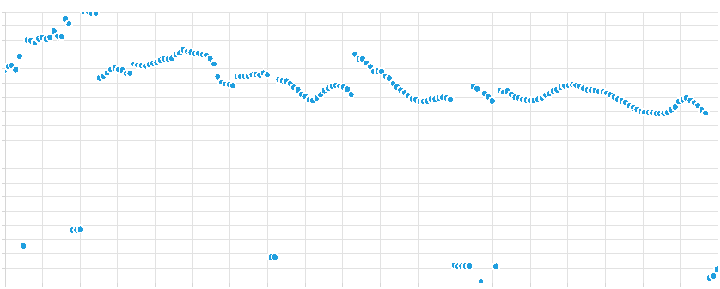
\includegraphics[scale=0.7]{zdanie_twierdzace.png}
\caption{Przebieg konturów intonacyjnych dla zdania „Intonacja w zdaniach twierdzących jest opadająca”. Próbkowanie 44kHz, estymacja z wykorzystaniem algorytmu YIN}
\end{figure}
\FloatBarrier
W pytaniach sytuacja ma się jednak inaczej, wbrew opinii powtarzanej w wielu źródłach, nie można wprost zakładać, że dla pytania intonacja będzie miała przebieg rosnący. Istnieje duża grupa pytań, dla których w tym przypadku intonacja również może mieć przebieg opadający lub będący połączeniem opadającego oraz rosnącego, w różnej kolejności. Powodowane jest to faktem, że w języku polskim rozróżniamy dwa rodzaje pytań. Wyróżnił je Kazimierz Ajdukiewicz w podręczniku „Logika Pragmatyczna” wydanym w 1965 roku.
Na podział ten składają się:
\begin{enumerate}
\item Pytania rozstrzygnięcia. Są to pytania, na które można udzielić odpowiedzi tak lub nie. Przykładem może być pytanie: „Czy byłeś dzisiaj w pracy?”  Cechują się silną antykadencją, umiejscowioną zazwyczaj w ostatnim wyrazie. Mogą występować również bez partykuły „czy”, na przykład pytanie „Mógłbyś to zrobić?” również jest pytaniem rozstrzygnięcia. Poprawna klasyfikacja takiej wypowiedzi na podstawie intonacji jest zadaniem stosunkowo prostym.
\item Pytania uzupełnienia. Nazywamy tak pytania, na które nie można udzielić odpowiedzi twierdzącej lub przeczącej. W wypowiedziach tych, akcent intonacyjny, mogący wskazywać, ze jest to pytanie kładziony jest na zaimek pytajny, będący najczęściej pierwszym wyrazem.

\begin{figure}[h]

\centering
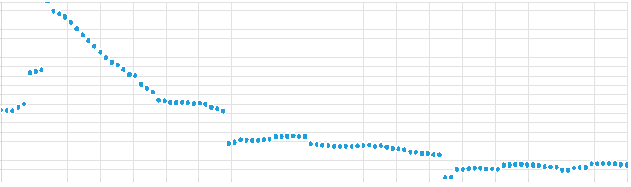
\includegraphics[scale=0.9]{pytanie_uzupelnienie.png}
\caption{Przykład pytania o uzupełnienie : „Jaką intonację ma to pytanie?”}

\end{figure}
\FloatBarrier
Silny wzrost intonacji występuje na samym początku sygnału, następnie widoczny jest niemal ciągły spadek.
Istnieją również pytania o uzupełnienie, dla których wzrost intonacji ma swoje miejsce na końcu wypowiedzi, obrazując typową antykadencję:
 \begin{enumerate}

\item Pytania odwrócone, np. W zeszłym roku byłem we Francji. A w Belgii? (= Kiedy byłeś w Belgii?) 
\begin{figure}[h]
\centering
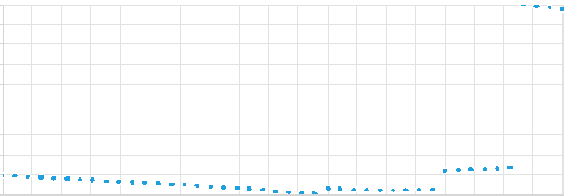
\includegraphics[scale=0.9]{pytanie_odwrocone.png}
\caption{Jest to pytanie odwrócone, które brzmi „A w Belgii?”}
\end{figure}
\FloatBarrier
\item Antykadencja występuje  także w pytaniach nawiązujących upewnienia. Występuje wówczas zarówno w  pytaniach o rozstrzygnięcie, jak i o uzupełnienie, a jej funkcją jest domaganie  się powtórzenia i potwierdzenia informacji, np. Byłem tam wczoraj. Kiedy?  Wczoraj."[  (Leokadia Dukiewicz, Irena Sawicka, "Fonetyka i fonologia", Kraków 1995) ]
\begin{figure}[h]

\centering
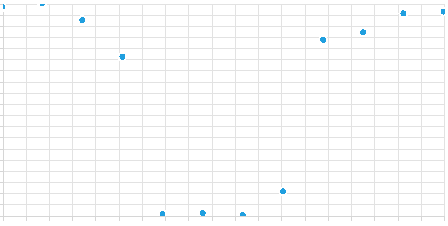
\includegraphics[scale=0.9]{kiedy.png}
\caption{Przykład pytania nawiązującego upewnienie : „Kiedy?”}
\end{figure}
\FloatBarrier
Przebieg intonacji dla takiego pytania jest opadająco-rosnący.
\end{enumerate}
\end{enumerate}
\section{Implementacja detekcji konturów częstotliwości podstawowej}
Celem praktycznym pracy jest stworzenie aplikacji desktopowej umożliwiającej wczytanie próbki zawierającej nagrane zdanie oraz dokonanie identyfikacji rodzaju tej wypowiedzi

\subsection{Język programowania oraz środowisko}
Pierwszym rozważanym zagadnieniem był wybór języka programowania oraz środowiska. Należało wziąć pod uwagę zawartość bibliotek związanych z przetwarzeniem dźwięku, oferowanych przez poszczególne języki.
Mimo rozpatrywania możlwości wielu języków, główny wybór zawarty był między Javą oraz C++. Dla obu języków dostępna jest mnogość gotowych funkcji wspierających pracę z dźwiękiem. Jako, że projekt zakładał stworzenie graficznego interfejsu użytkownika, 
konieczny był również wybór odpowiedniego środowiska, umożliwiającego stworzenie takiej aplikacji. Dla języka Java jako środowisko spełniające takie wymagania postrzegany był Eclipse wraz z frameworkiem JavaFx. Nie posiadają one wbudowanych pomocy do pracy z próbkami dźwięku, lecz dla Javy stworzone zostało
Java Sound API. API te zawiera podstawowe funkcjonalności, jest pomocne przy wczytywaniu plików wav. W celu korzystania z tego rozszerzenia, należy je po prostu zaimportować. Dla  C++ sytuacja wygląda zgoła inaczej. Pracując z tym językiem, można korzystać z możliwości obszernego frameworka - Qt. Oferuje on wiele węwnetrznych klas ułatwiających pracę z dźwiękiem. Działają one niskopoziomowo, wszelkie zadania wykonywane są dużo szybciej niż w przypadku Javy.  System sygnałów i slotów, charakterystyczny dla Qt, jest bardzo wygodny przy wczytywaniu kolejnych próbek dźwieków. Umożliwia to aktualizowanie wykresów przedstawiających odczytane lub obliczone wartości na bieżąco. Dodatkowo, tworzenie graficznego interfejsu użytkownika w tym środowisku jest bardziej intuincyjne. Biorąc pod uwagę argumenty, wybór padł na język C++ z wykorzystaniem frameworka Qt.

\subsection{Opis możliwości aplikacji}
W pierwotnym założeniu aplikacja miała umożliwiać nagrywanie wypowiedzi, która następnie miała zostać poddana rozpoznaniu. Jednak w trakcie implentacji nie sposób było nie zauważyć, że znacznie lepsze wyniki rozpoznania są uzyskiwane, gdy do programu zostanie wczytana wypowiedź nagrana zewnętrznym programem, oraz poddana w nim obróbce wstępnej. Spowodowało to porzucenie tej funkcjonalności, jako że nie jest ona konieczna do osiągnięcia zakładanego celu, jakim jest poprawne rozpoznawanie rodzaju wypowiedzi.

Aplikacja umożliwa wczytanie pojedynczego nagrania lub całego katalogu z nagraniami. Program wyświetla nazwę wczytanego pliku, oraz rodzaj zdania do jakiego dana wypowiedź została sklasyfikowana. Po kliknięciu w tabeli na wybrany wiersz, a następnie po kliknięciu na jeden z dowolnych przycisków w dolnym pasku, program wyświetli na wykresie odpowiednio energię nagrania, przebieg widma, przebieg wartości próbki w dziedzinie czasu (waveform) lub przebieg wyestymowanej częstotliwości podstawowej.
\subsection{Wczytanie próbki}
Pierwszym krokiem na drodze do rozpoznania rodzaju zdania, jest wczytanie calego nagrania przez program. Wykonuje sie to z wykorzystaniem mozliwosci oferowanych przez Qt. Framework oferuje do tego klase QAudioDecoder. 
Nagranie jest wczytywane w 100 milisekundowych fragmentach. Jako że częstotliwość próbkowania wynosi 44100Hz, na jeden fragment przypada 4410 wartości. Każda częśc jest odczytana jako obiekt klasy QAudioBuffer. Wektor typu QAudioBuffer zawiera cale wczytane nagranie.
\begin{lstlisting}
std::vector<QAudioBuffer>audioBuffers;
QAudioDecoder *audioDecoder;
\end{lstlisting}
\begin{lstlisting}
audioDecoder = new QAudioDecoder();
connect(audioDecoder, SIGNAL(bufferReady()), this, SLOT(readBuffer()));
connect(audioDecoder,SIGNAL(finished()),this,SLOT(decodingFinished()));
audioDecoder->start();
\end{lstlisting}
Po wczytaniu kazdej z ramek emitowany jest sygnal. Laczac sygnal ze slotem, mozliwe jest przechwycenie aktualnie wczytanych wartosci, zanim zostana zastapione wartosciami kolejnej ramki.
Zostaja one dodane do wektora ramek.
\begin{lstlisting}
void MainWindow::readBuffer()
{
    audioBuffers.emplace_back(audioDecoder->read());
}
\end{lstlisting}
Gdy cale nagranie zostanie odczytane, QAudioDecoder emituje sygnal finished(). Po jego przechwyceniu, a wiec otrzymaniu informacji o zakonczeniu dekodowania, program umieszcza w jednym wektorze próbki ze wszystkich 100 milisekundowych buforów.

\begin{lstlisting}[caption={Funkcja dodająca do wektora wszystkie odczytane próbki},label={lst:label},language=C++]

void MainWindow::putValuesIntoVector()
{
    sampleRate = audioBuffers[0].format().sampleRate();
    frameSize = audioBuffers[0].format().sampleRate()/40;
    
    for (QAudioBuffer audioBuffer : audioBuffers)
    {
        const qint16 *data = audioBuffer.constData<qint16>();
        for(int j=0;j<audioBuffer.sampleCount();j++)
        {
              wholeBuffer.emplace_back(data[j]);
        }
        delete data;
    }
}
\end{lstlisting}
W powyższej funkcji, najpierw pobierana jest ilość próbek przypadających na jedną sekundę, oraz na 25 milisekundową ramkę. Następnie wartości kolejno z każdego obiektu typu QAudioBuffer, znajdującego się w wektorze audioBuffers, są dodawane do wektora wholeBuffer. Jest to wektor przechowujący zmienne
zmiennoprzecinkowe, o podwójnej precyzji, tj.double.

\subsection{Ekstrakcja tonu podstawowego}
W pierwotnym założeniu program, poza estymacją częstotliwości podstawowej miał również dokonywać ekstrakcji niskopoziomowych cech.
W toku implementacji zostały one jednak pominięte, z powodu posiadania małego wpływu na cel pracy. 
Pierwszym zagadnieniem, które powinno być rozważone, jest długość fragmentów sygnału, na które powinien być podzielony.
Sygnały mowy nie są sygnalami stacjonarnymi, co oznacza, że ich częstotliwość istotnie zmienia się w czasie, znacznie obniżając dokładność obliczeń, opierających się na rezultatach transformaty Fouriera.
W przetwarzaniu mowy korzystne jest dzielenie sygnału na części, celem uzyskania fragmentów sygnału bliskich byciu stacjonarnymi.
Głośnia, odpowiedzialna za zmiany częstotliwości głosu, nie zamyka i nie otwiera się natychmiastowo, co oznacza, że w małych odstępach czasu wartości częstotliwości są do siebie zbliżone.
Odpowiednio dzieląc sygnał możliwe jest uzyskanie krótszych  quasi-stacjonarnych fragmentów. Proces ten nazywa się ramkowaniem.
\subsubsection{Ramkowanie oraz ekstracja wartości F0}
Sygnał najczęśniej dzielony jest na 20-50ms ramki. W tym projekcie ustalona długość ramki wynosi 25ms. Oznacza to, że każda ramka składa się z 1102 wartości.
Pojawia się jednak problem związany z wartościami brzegowymi. Dzieląc sygnał na przystające do siebie, lecz nie zachodzące na siebie ramki istnieje duże ryzyko nie wykrycia pewnych cech, które mogą znajdować się pomiędzy dwoma kolejnymi ramkami. 
Taka sytuacja mogłaby wystąpić podczas analizy sygnału w celu wykrycia konturów częstotliwości podstawowej. Jeżeli relatywnie krótki kontur zaczynałby się w jednej ramce i kończył w drugiej, mógłby nie zostać wykryty.
Rozwiązaniem jest nakładanie ramek na siebie (overlapping).Określona część każdej ramki, zawarta jest również w ramce kolejnej. Najczęściej jest to 20-50\% segmentu.
\begin{figure}[h]

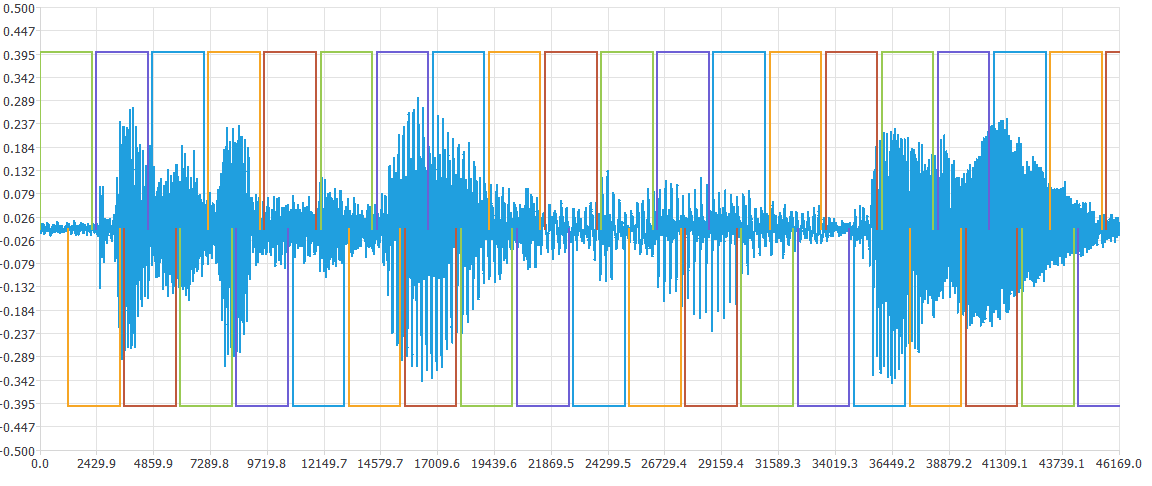
\includegraphics[scale=0.7]{overlapping.png}
\caption{Zobrazowany podział sygnału na ramki wraz zastosowaniem 30-procentowego overlappingu. Opracowanie własne}
\end{figure}
\FloatBarrier
Do ekstrakcji cech niskopoziomowych 30 procentowe nakładanie się ramek jest wystarczające. Jednak algorytm YIN, wykorzystany w projekcie do estymacji F0, wymaga znacznie większego zachodzenia fragmentów na siebie. W tym przypadku 90\% danej ramki znajduje się również w ramce kolejnej.
Oznacza to, że ramki przesuwane są jedynie o 2,5ms. Spowodowane jest to faktem, że algorytm YIN opiera swoje działanie na funkcji autokorelacji.
Do ekstrakcji cech stworzona została klasa ExtractionHelper.
\FloatBarrier
\begin{figure}[h]
\centering
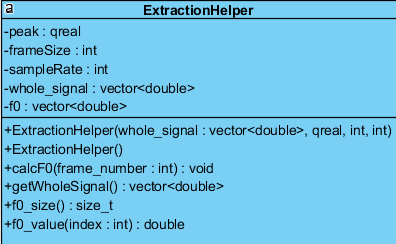
\includegraphics[scale=0.9]{featuresExtractor.png}
\caption{Klasa stworzona w celu ekstracji F0, obliczenia energii sygnału oraz przechowywania tych wartości}
\end{figure}
\FloatBarrier

\begin{lstlisting}[caption={Przedstawienie sposobu dokonywania podziału na ramki, wraz z zastosowaniem overlappingu},label={lst:label},language=C++]
void ExtractionHelper::calcF0(int numberOfFrames)
{

   int numberOfShifts=10;

   Yin m_yin(frameSize, sampleRate);


   int frameStartIndexAfterShifting = 0;
   int shift= frameSize/numberOfShifts;

   while(frameStartIndexAfterShifting < (whole_signal.size()))
   {
       double *shift_frame =new double [frameSize];
       int index=0;
       frameStartIndexAfterShifting +=shift;
       for(int k=frameStartIndexAfterShifting;k<frameStartIndexAfterShifting+frameSize;k++)
       {
           if(k>=whole_signal.size())
              shift_frame[index] = 0;
           else
              shift_frame[index] = whole_signal.at(k);
           index++;
       }
       Yin::YinOutput f0_struct=m_yin.process(shift_frame);
       if (f0_struct.f0 <F0_MAX && f0_struct.f0 >F0_MIN)
           f0.emplace_back(f0_struct.f0);
       else
           f0.emplace_back(0);
       delete shift_frame;
   }

}
\end{lstlisting}
W funkcji wykorzystywana jest klasa Yin, pochodząca z ogólnodostępnej implementacji algorytmu YIN. Konstruktor obiektu tej klasy jako argumenty przyjmuje długość pojedynczej ramki oraz częstotliwośc próbkowania. W tym przypadku wartości te wynoszą kolejno 1102 i 44100. 
W ciele funkcji calcF0 obiekt ten będzie wykorzystywany do estymacji konturów F0 dla pojedynczych ramek. 
Z racji zastosowania wysokiego overlappingu, proces dzielenia sygnału na fragmenty nie wygląda jak typowe ramkowanie. Okno sygnału przeznaczone do estymacji będzie przesuwane jedynie o 2,5ms.
W tym celu zadeklarowane zostały dwie zmienne, frameStartIndexAfterShifting przechowuje początkowy indeks obecnie przetwarzanej ramki, a zmienna shift przechowuje wartość pojedynczego przesunięcia.
Warunkiem kończącym działanie głównej pętli funkcji jest przekroczenie przez początkowy indeks ramki rozmiaru całego sygnału. Oznacza to, że końcowa ramka może być dowolnie mała.
W wewnętrznej pętli wartości rozpatrywanej ramki są przypisywane do dynamicznie zadeklarowanej tablicy. Jeżeli indeks tej pętli przekroczy rozmiar całego sygnału, reszta pól tablicy wypełniona jest zerami. Powodem tego jest wymaganie implementacji algorytmu YIN, aby wszystkie ramki miały jednakowy rozmiar.
Po zakończeniu estymacji wartości F0 dla danej ramki, wartość ta jest dodawana do wektoru jeżeli mieści się w zdefiniowanym zakresie. Musi być większa niż 60 i mniejsza niż 450. W przeciwnym razie do wektoru zostanie dodana wartość zerowa. Po obliczeniach zadeklarowana dla ramki pamięć zostaje zwolniona.
\subsection{Wykrywanie konturów}
Wszystkie wyestymowane wartości częstotliwości podstawowej na tą chwilę przechowywane są w jednym wektorze. Aby umożliwić analizę przebiegu intonacji, konieczne jest wydzielenie poszczególnych konturów. Segmentacji można dokonać analizując wartości pod kątem wartości odstających.
 Do tego celu zostały stworzone dwie klasy.
 \FloatBarrier
\begin{figure}[h]
\centering
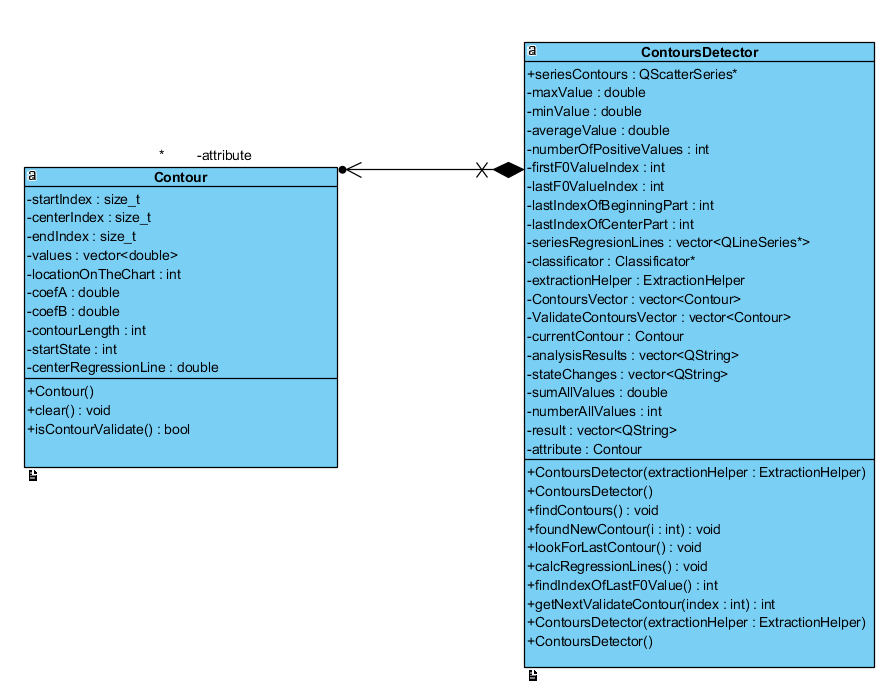
\includegraphics[scale=0.9]{contourDetector.png}
\caption{Klasy stworzone do wykrycia poszczególnych konturów intonacyjnych, na podstawie wszystkich wartości F0}
\end{figure}
\FloatBarrier
Dla każdej ze zmiennych istnieją funkcje typu get i set, odpowiednio zwracające wartość zmiennej oraz przypisujące dana wartość. Zostały one pominięte w celu zwiększenia czytelności diagramów.
Główna funkcjonalność zawarta jest w funkcji findContours() w klasie ContoursDetector. Wykryte kontury będą umieszczane jako obiekty typu Contour, w wektorze contoursVector. W wektorze tym będą również umieszczane fragmenty z wartościami zerowymi, dla których nie wykryto występowania intonacji. Będą one pomijane w dalszej analizie, dodawane są w celu ułatwienia przejrzystego wyświetlania konturów na wykresie, w miejscu w którym rzeczywiście się znajdują.

\begin{lstlisting}[caption={Początkowa faza funkcji wykrywającej kontury},label={lst:label},language=C++]
#define TRANSITION 15

void ContoursDetector::findContours()
{
    currentContour.setStart(1);
    lastValueIndex = findIndexOfLastF0Value();
    for(size_t i=1;i<extractionHelper.f0_size();i++)
    {
        double value =extractionHelper.f0_value(i);
        double previousValue = extractionHelper.f0_value(i-1); 
        seriesContours->append(i,value);
        if (value > maxValue) maxValue = value;
        if (value < minValue && value > F0_MIN) minValue = value;
        if(std::abs(value - previousValue) > TRANSITION)
        {
            currentContour.setEnd(i-1);
  	    currentContour.setCenter();    
            foundNewContour();
            currentContour.setStart(i);
            currentContour.addValue(value);
        }
        else
        {
            currentContour.addValue(value);
        }
    }
\end{lstlisting}
Początkowy indeks pierwszego konturu jest ustawiony jako 1. Główna pętla przebiega po wszystkich wyestymowanych wartościach tonu podstawowego. Oprócz poszukiwania konturów, wartości są również sprawdzane pod kątem wykrycia wartości maksymalnej i minimalnej. Funkcja wykrywanie danego konturu za zakończone, gdy aktualnie rozpatrywana wartość rózni się od poprzedniej o 15 jednostek. Metodą obserwacji ustalono taki przeskok za wystarczający do stwierdzenia, że dana wartość należy już do nowego konturu. Poprzedzający indeks jest uznawany za koniec danego konturu. Aktualny licznik pętli zostaje przekazany do funkcji foundNewContour. Z uwagi na obszerność tej funkcji, będzie ona omawiana fragmentami.
\begin{lstlisting}[caption={Funkcja zajmująca się analizą wstępną wykrytego konturu},label={lst:label},language=C++]
void ContoursDetector::foundNewContour()
{
    if (!currentContour.isContourValidate())
    {
        currentContour.clear();
        return;
    }
    
    if (lastIndexOfFirstPart == 0)
    {
        firstValueIndex = currentContour.getStartIndex();
        double occurenceRange = lastValueIndex-firstValueIndex;
        lastIndexOfFirstPart = currentContour.getStartIndex()+occurenceRange/4;
        lastIndexOfCenterPart = lastValueIndex - occurenceRange/4;
    }
    
    if (currentContour.getCenter() < lastIndexOfFirstPart)
       currentContour.setLocation(BEGINNING);
    else if (currentContour.getCenter() < lastIndexOfCenterPart)
        currentContour.setLocation(CENTER);
    else
        currentContour.setLocation(END);
            
\end{lstlisting}
Najpierw kontur jest poddawany walidacji. Sprawdzane jest, czy nie występują w nim wartości zerowe oraz czy jego długość jest większa niż 1. Przyjęta implementacja segmentacji traktuje wartości zerowe jako przerwy między konturami i nie powinny one być dodawane do wektoru przechowującego wykryte kontury. Do określania czy dany obiekt jest przerwą między konturami, wystarczy sprawdzić jego pierwszą wartość.
Metodą obserwacji zauważono, że kontury składające się tylko z jednej wartości, często są błędami estymacji, lub powstają w wyniku róznego rodzaju zanieczyszczeń w nagraniu. Mogą zaburzać wyniki późniejszej klasyfikacji, dlatego są pomijane.
\begin{lstlisting}[caption={Funkcja dokonująca walidacji konturu},label={lst:label},language=C++]
    bool isContourValidate()
    {
        if (values.size()<2) return false;
        if (values.at(0) == 0)  return false;
        return true;
    }
\end{lstlisting}
Póżniejsza analiza konturów w celu wykrycia rodzaju danego zdania, oparta jest w dużej mierze na położeniu danego konturu w przestrzeni przebiegu całej intonacji. Przebieg intonacji zawiera wartości od pierwszego poprawnego konturu do ostatniego. Wykres jest dzielony na 3 części. Na część początkową oraz końcową przypada po 25\% całości, podczas gdy część środkowa zawiera pozostałą połowę.
W celu przydzielenia konturom odpowiedniej lokalizacji, używane są zmienne typu całkowitego, lastIndexOfFirstPart oraz lastIndexOfCenterPart. Wyznaczają one końce początkowej oraz środkowej części. Następnie, w zależności od położenia środka konturu, zostaje mu przypisane odpowiednie makro, zawierające informację o lokalizacji konturu.
 \FloatBarrier
\begin{figure}[h]
\centering
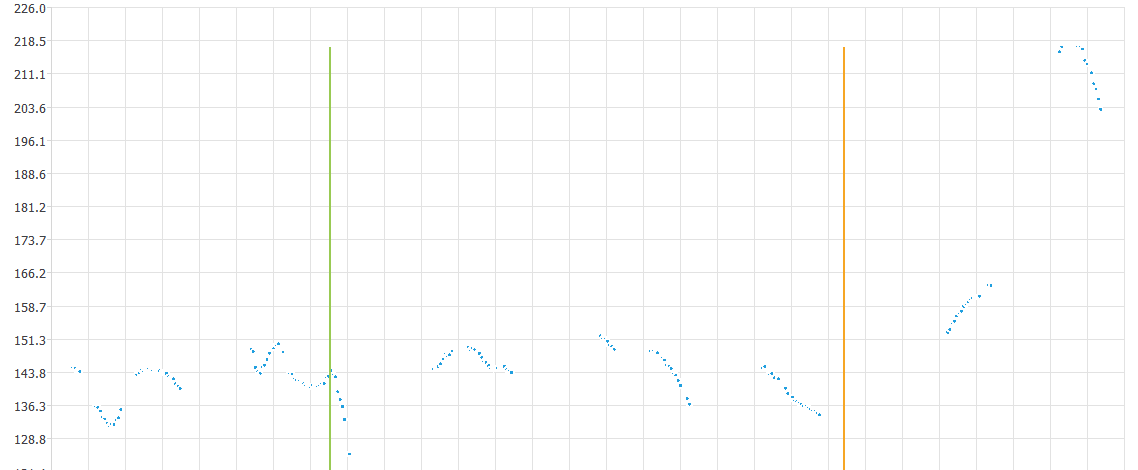
\includegraphics[scale=0.7]{podzial_wykresu.png}
\caption{Przykład podziału przebiegu intonacji na 3 części}
\end{figure}
\FloatBarrier
\begin{lstlisting}
     if (ContoursVector.size()>0)
    {
        if ((currentContour.getFirstValue()
        	-ContoursVector.back().getLastValue())
                >(currentContour.getFirstValue()/6))
        {
            currentContour.setStartState(GROWTH);
        }
        else if ((ContoursVector.back().getLastValue() 
        	- currentContour.getFirstValue())
                 >(ContoursVector.back().getLastValue()/4))
        {
            currentContour.setStartState(DROP);
        }
    }
    ContoursVector.push_back(currentContour);
    currentContour.clear();
}
\end{lstlisting}
W dalszej części kodu funkcji foundNewContour, dokonywana jest analiza położenia danego konturu względem poprzednika. Jeżeli początkowa wartość analizowanego konturu jest znacząco mniejsza lub większa od ostatniej wartości konturu poprzedzającego, zapisywana jest informacja o gwałtownym przeskoku w przebiegu intonacji.
 \FloatBarrier
\begin{figure}[h]
\centering
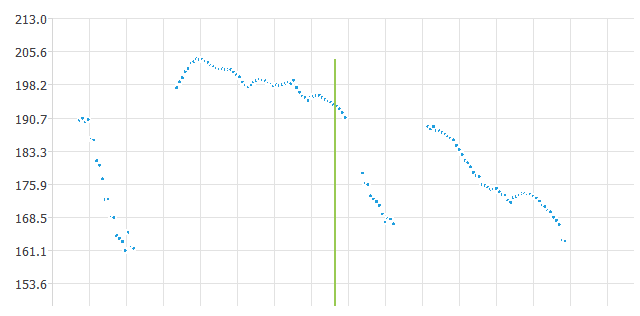
\includegraphics[scale=0.7]{przeskok.png}
\caption{Przykładowy przeskok(wzrost) między pierwszym i drugim konturem, zlokalizowanymi w początkowej części}
\end{figure}
\FloatBarrier
Następnie kontur zostaje dodany do wektoru, a zmienna currentContour zostaje wyczyszczona w celu poszukiwania kolejnego konturu.
\section{Analiza wykrytych konturów}
\end{document}